\documentclass{article}
\usepackage[utf8]{inputenc}
\usepackage{graphicx}% Include figure files
\usepackage{hyperref}  
\usepackage{color}
\usepackage{verbatim}
\usepackage{amsmath}
\usepackage{polski}
\usepackage[section]{placeins}

\title{MPiS - Zadanie 1}
\author{Michał Łukomski}
\date{\today}

\begin{document}

\maketitle

\section{Szacowanie wartości całek}
Całki szacowano za pomocą metody Monte Carlo za pomocą wzoru:
\begin{equation}
    \int_{a}^{b} f(x) dx \approx \frac{C}{n} (b-a) M
\end{equation}
gdzie $C$ to liczba punktów, które zalazły się w obszarze pod krzywą, $n$ to liczba losowanych punktów, $M$ to wartośc większa niż maksimum funkcji $f(x)$ w przedziale $[a,b]$.

\begin{figure}[!h]
    \centering
    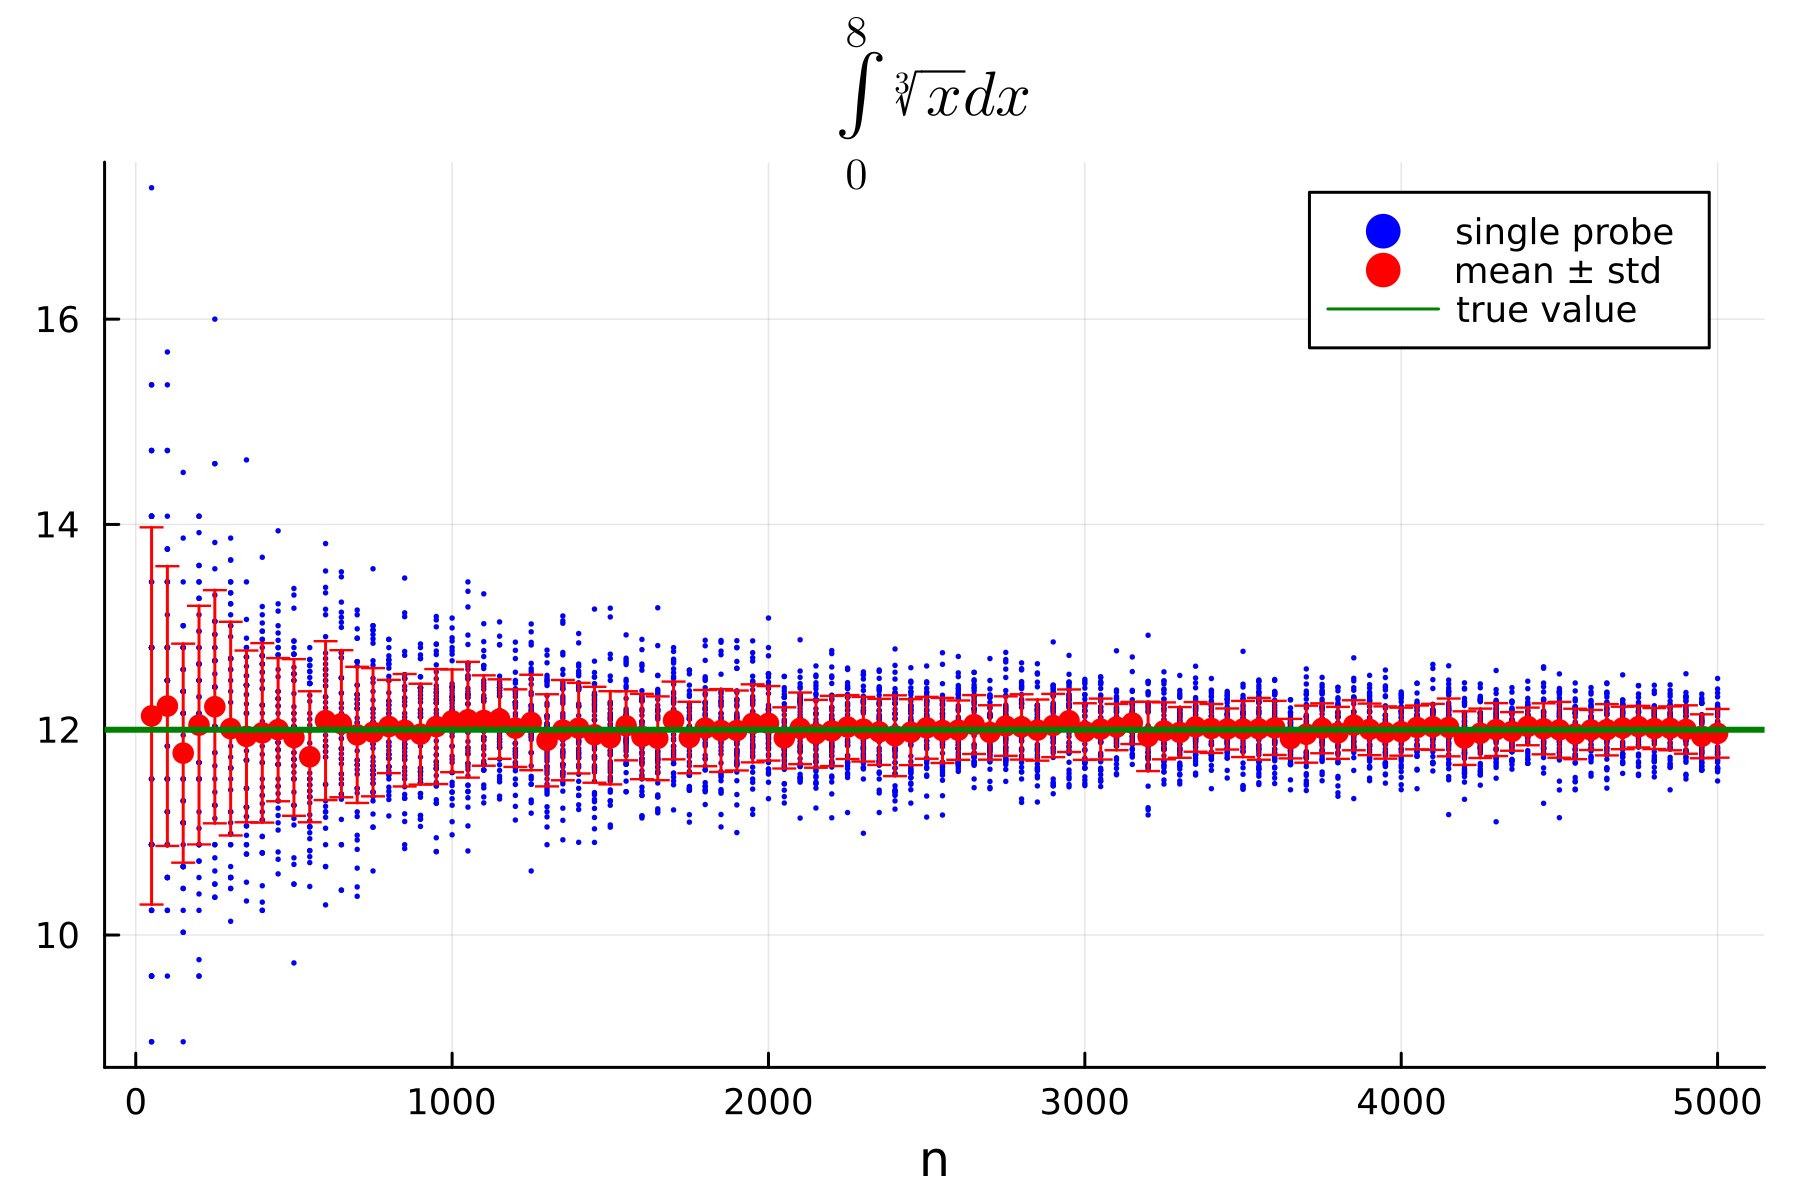
\includegraphics[width=\linewidth]{results/z1_1.png}
    \caption{Wyniki eksperymentów dla całki $\int_0^8 \sqrt[3]{x} dx$. Dla $n \in {50, 100, \dots, 5000}$, dla każdego $n$ wykonano $k=50$ niezależnych powtórzeń algorytmu. Niebieski - wynik pojedynczej aproksymacji, czerwony - średnia z $k$ powtórzeń wraz z odchyleniem standardowym jako słupkiem błędu, zielony - wartość dokładna całki.}
\end{figure}

\begin{figure}[!h]
    \centering
    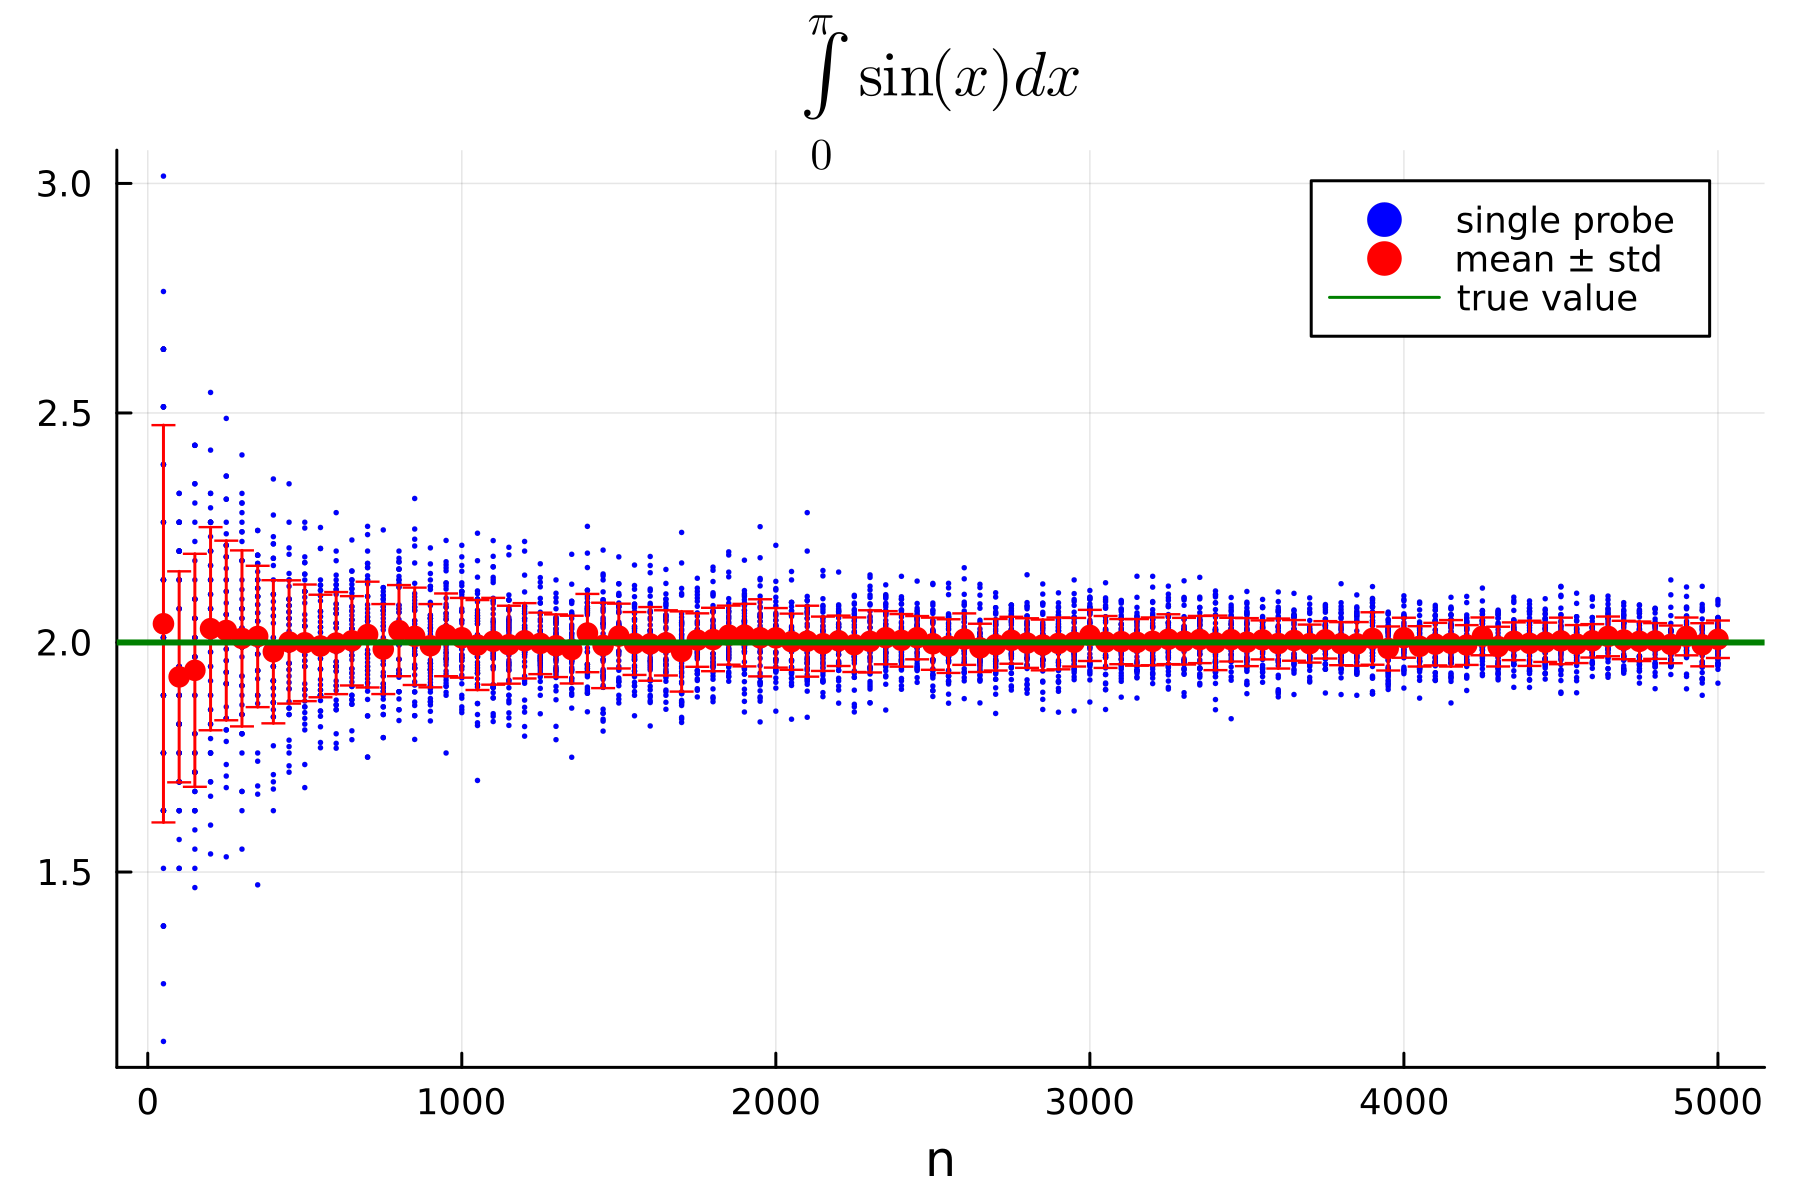
\includegraphics[width=\linewidth]{results/z1_2.png}
    \caption{Wyniki eksperymentów dla całki $\int_0^{\pi} \sin(x) dx$. Dla $n \in {50, 100, \dots, 5000}$, dla każdego $n$ wykonano $k=50$ niezależnych powtórzeń algorytmu.}
\end{figure}

\begin{figure}[!h]
    \centering
    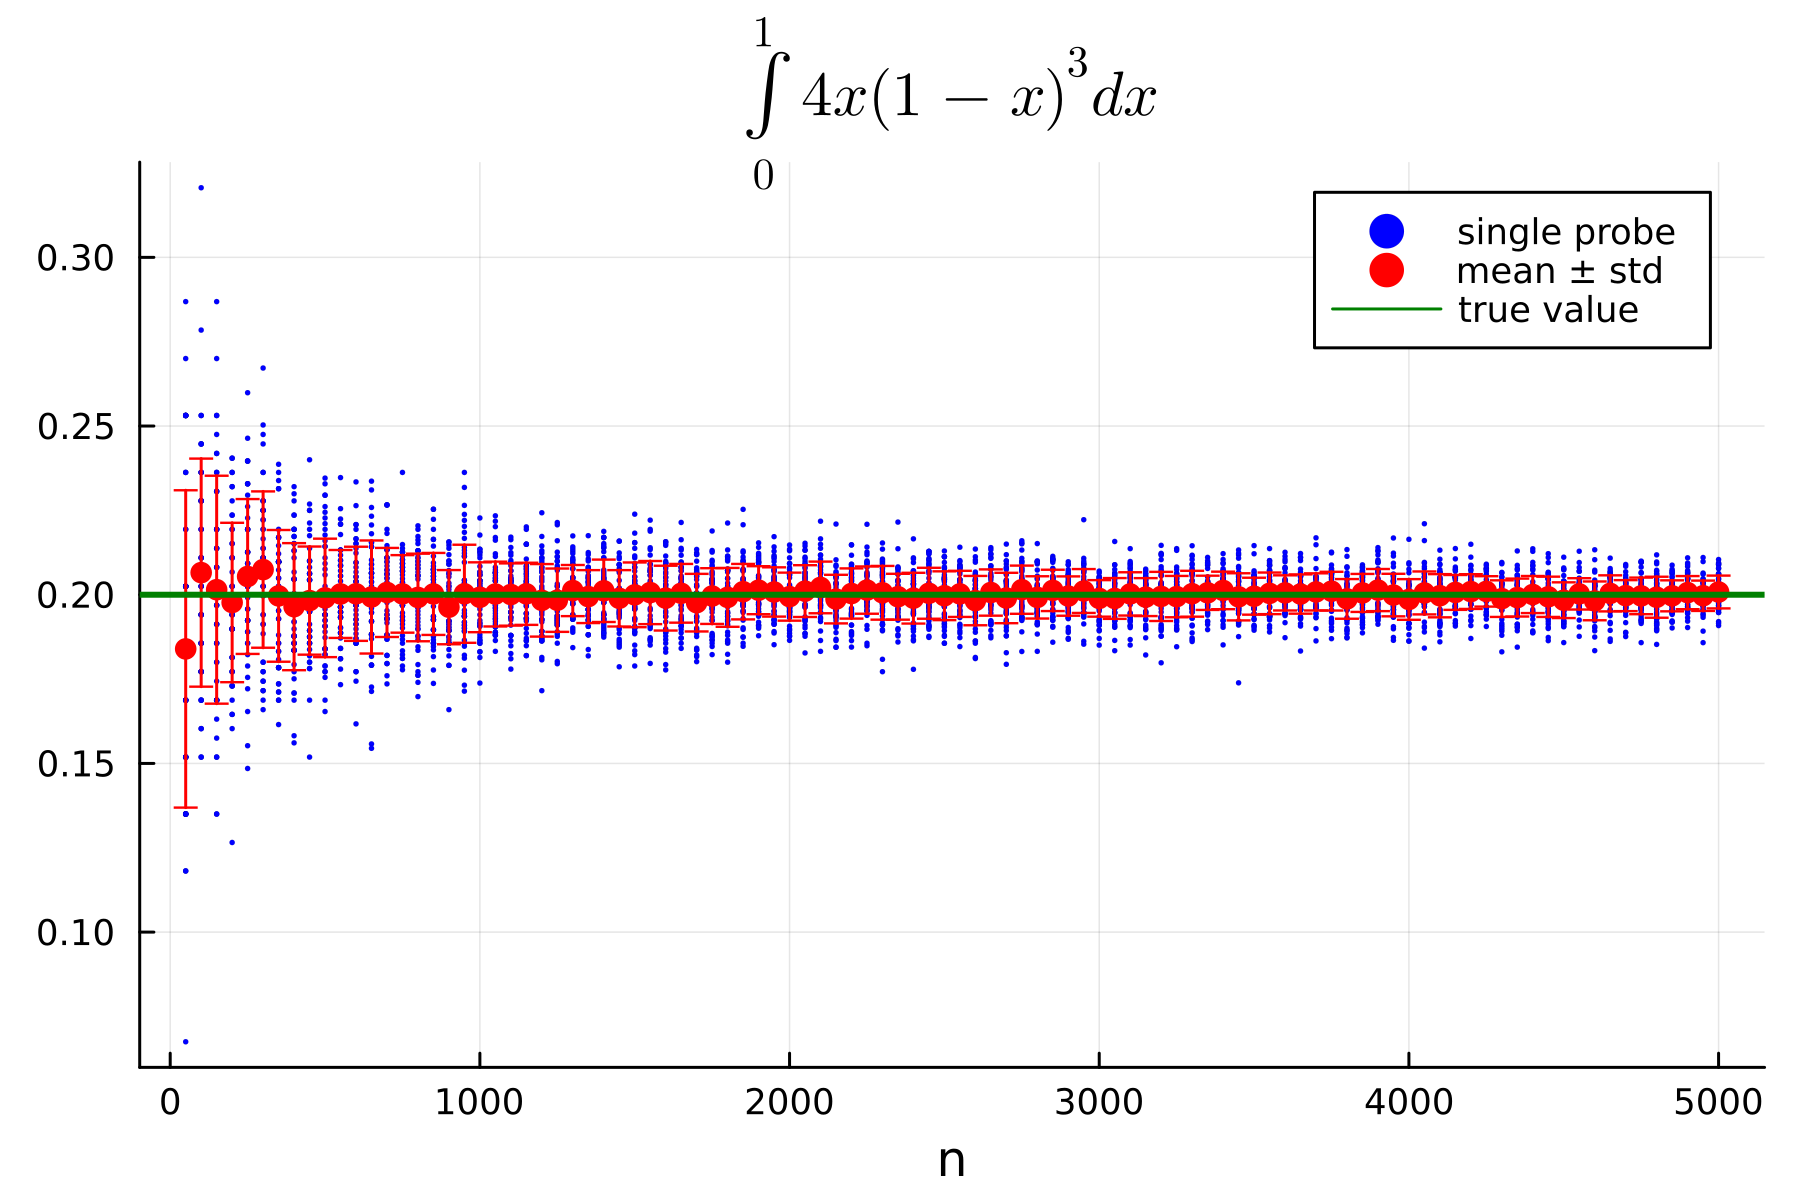
\includegraphics[width=\linewidth]{results/z1_3.png}
    \caption{Wyniki eksperymentów dla całki $\int_0^1 4x(1-x)^3 dx$. Dla $n \in {50, 100, \dots, 5000}$, dla każdego $n$ wykonano $k=50$ niezależnych powtórzeń algorytmu.}
\end{figure}



\section{Aproksymacja liczby $\pi$}

\begin{figure}[!htbp]
    \centering
    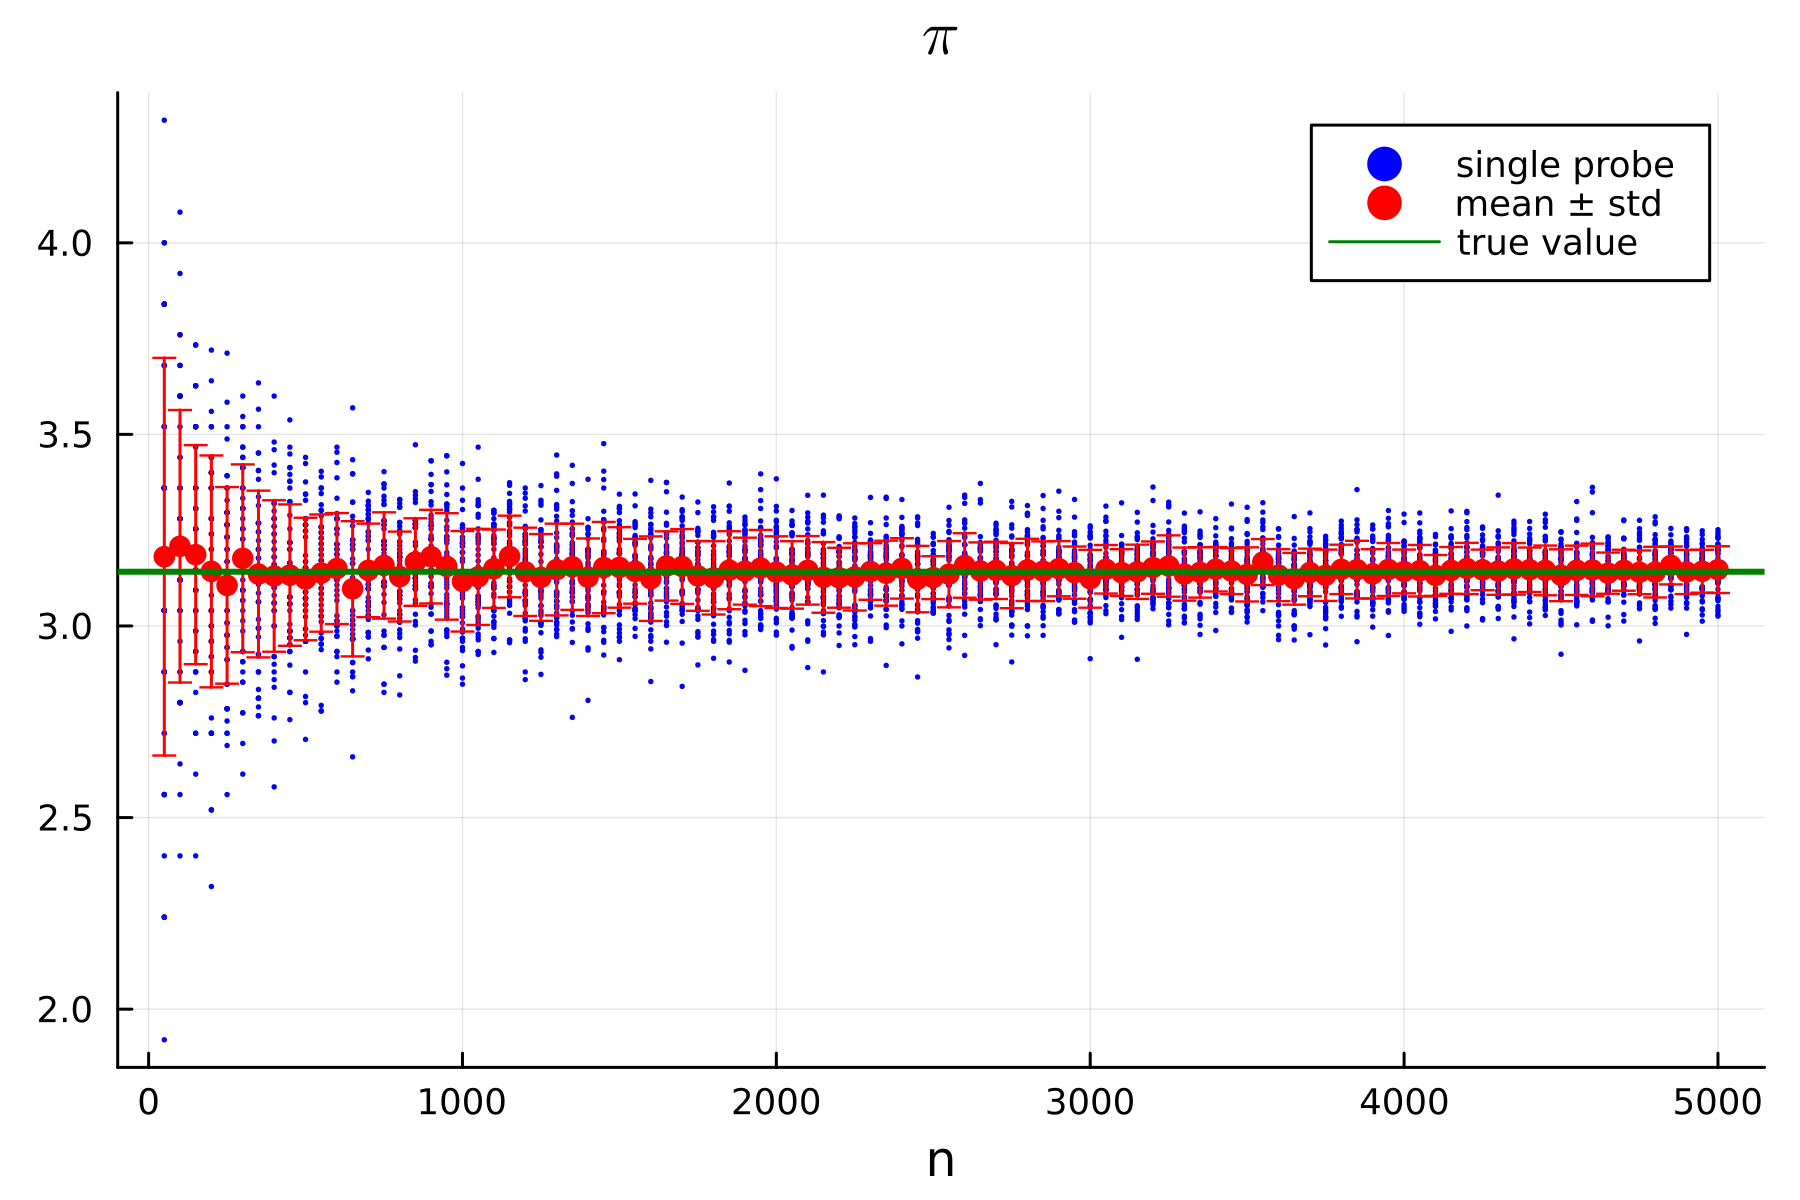
\includegraphics[width=\linewidth]{results/z1_4.png}
    \caption{Wyniki eksperymentów dla wyznaczania aproksymacji liczby $\pi$. Liczono w tym celu całkę $\int_{-1}^{1} 2\sqrt{1-x^2} dx$, której wartość dokładna wynosi $\pi$. Dla $n \in {50, 100, \dots, 5000}$, dla każdego $n$ wykonano $k=50$ niezależnych powtórzeń algorytmu.}
\end{figure}

\section{Wnioski}
Jak widać na powyższych wykresach im więcej $n$ punktów wylosowano, tym dokładniejsze wyniki uzyskano. Czyli gdy $n\rightarrow \infty$, to wartość całki aproksymowanej dąży do wartości dokładnej, a odchylenie standardowe niezależnych powtórzeń algorytmu dąży do 0.

Warto też zwrócić uwagę, że średnie po niezależnych powtórzeniach algorytmu są generalnie bardziej zbliżone do wartości dokładnej całki, niż pojedyncze wyniki, a wynika to z tego, że w przypadku pojedynczego wyniku losowanych jest tylko $n$ punktów, a średnia z $k$ powtórzeń algorytmu to wynik z $kn$ (czyli $50 n$ punktów w tym przypadku). Wynika to bezpośrednio ze wzoru:
\begin{equation}
    \begin{split}
        I_{mean} &= \frac{1}{k} \sum_{i=1}^k I_i \\
        &= \frac{1}{k}\sum_{i=1}^k \frac{C_i}{n} (b-a) M \\
        &= \frac{1}{kn} (b-a) M \sum_{i=1}^k C_i \\
        &= \frac{C_{mean}}{kn} (b-a) M
    \end{split}
\end{equation}

Jeśli chodzi więc o wynik końcowy to nie ma znaczenia czy wykonamy średnią z $k$ powtórzeń po $n$ punktów, czy po prostu wylosujemy $kn$ punktów i policzymy wartość całki, to dostaniemy wynik z taką samą dokładnością. Jednak w pierwszym przypadku możemy dostać informację o rozrzucie wyników, a w drugim nie.

Eksperyment wykonano w języku Julia 1.7.2, jako generator liczb losowych wykorzystano Xoshiro256++ - domyślnego generatora języka Julia.
Wartości dokładne całek zostały obliczone za pomocą programu WolframAlpha.

\end{document}
